\subsection{Descripción del filtro}

El filtro de color es una transformación sobre imágenes a color que tiene el efecto de decolorizar o pasar a escala de grises todos los píxeles de la entrada cuyo color no esté dentro de un rango de colores especificado. En la figura \ref{fig:filtro-color-ejemplo} se observa un ejemplo de funcionamiento típico.

\begin{figure}[h]
\begin{center}
  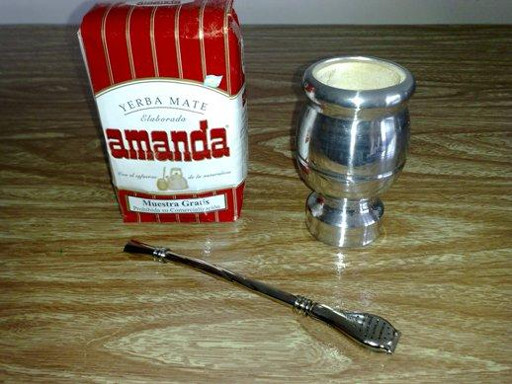
\includegraphics[scale=0.4]{secciones/filtro_color/imagenes/matecocido.jpg}
  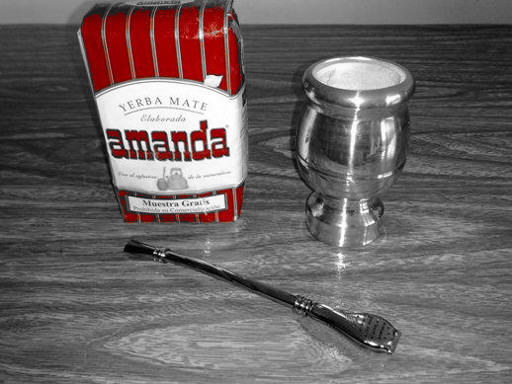
\includegraphics[scale=0.4]{secciones/filtro_color/imagenes/matecocido-fcolor.jpg}
\end{center}
\caption{Imagen antes y después de aplicar el filtro de color con color principal rojo.}
\label{fig:filtro-color-ejemplo}
\end{figure}

La forma en la cual se especifica el rango de colores que deberá permanecer inmutado es mediante la elección de un color principal, cuya codificación RGB se denota con (\param{rc}, \param{gc}, \param{bc}), y un parámetro umbral \param{threshold}. Una vez determinados estos valores, un píxel de la imagen fuente será actualizado por el filtro únicamente si cumple:


\begin{equation} \label{filtro-color-condicion}
\vectornorm{(r, g, b) - (rc, gc, bc)} > threshold 
\end{equation}

donde (\param{r}, \param{g}, \param{b}) es la codificación en RGB del píxel. En particular, de cumplirse esta condición, los tres canales se actualizan de la siguiente forma:

$$ r' = b' = g' = \frac{r + g + b}{3} $$

De esta última expresión se desprende que el color de los píxeles alterados pasa a estar en la escala de grises, ya que los tres canales toman igual valor. Como una observación adicional, queda claro mediante esta especificación que el filtro actúa de forma localizada en sobre cada píxel; su suceptibilidad a ser modificado y su nuevo valor dependen únicamente de su propio valor, y no del de sus vecinos.

\subsection{Implementación en lenguaje C y lenguaje ensamblador}

La implementación en C del filtro se realizó de la forma más sencilla e intuitiva posible; mediante un ciclo que visita una vez a cada píxel de la imagen, de izquierda a derecha y de arriba a abajo, evaluando la condición y modificando su valor de ser necesario. Como única optimización elemental, se modificó la condición (\ref{filtro-color-condicion}) por la siguiente condición equivalente:

$$\vectornorm{(r, g, b) - (rc, gc, bc)}^2 = (r - rc)^2 + (g - gc)^2 + (b - bc)^2 > threshold^2$$

La modificación evita el cálculo de una raíz cuadrada, sin incurrir en el riesgo de exceder el rango del tipo de datos utilizado ya que el máximo \param{threshold} que no hace a la condición trivialmente falsa es $\sqrt{195075} \approx 441$ (el valor máximo que puede tomar la expresión de la izquierda es $255^2 + 255^2 + 255^2 = 195075$), por lo que cualquier valor mayor se puede reducir a $442$.

La implementación en lenguaje ensamblador mantiene esencialmente el mismo procedimiento, con la salvedad de que fue adaptado para procesar cuatro píxeles en simultáneo mediante el uso de operaciones SIMD. Se recorre la matriz en el mismo órden descripto previamente, realizando lecturas de 16 bytes por iteración (equivalente a 5 píxeles y un byte sobrante).

La necesidad de limitar el procesamiento simultáneo a cuatro píxeles se desprende del hecho de que, como se dijo antes, la expresión que mide la distancia entre un píxel y el color principal puede tomar valores en el rango $0, ... \,195075$. Este último valor no cabe en un entero de 16 bits, precisándose un \tipo{double word} para almacenar ese resultado temporal; esto implica un total de hasta cuatro valores de distancia en un registro XMM. Por esta razón, además sería similar trabajar con el tipo de datos \tipo{float} ya que también caben hasta cuatro por registro de 128 bits.

De esta forma, el procedimiento realizado en cada iteración consiste en (para cada uno de los cuatro píxeles en simultáneo) comparar el valor de la distancia con el \param{threshold}, y calcular el promedio de los tres canales, actualizando luego sus valores según la siguiente expresión informal:

$$\text{valor\_original} \land \lnot \text{cumple\_condicion} + \text{promedio} \land \text{cumple\_condicion}$$

Esto permite expresar el equivalente a una expresión del tipo \textbf{if}-\textbf{then}-\textbf{else}, en el lenguaje del procesamiento simultáneo. El cómputo de los flags con el resultado de las comparaciones y del promedio se puede describir mediante el pseudo-código de la figura \ref{fig:pseudocodigo-filtro-color}.

\begin{figure}[h]
	\begin{mdframed}
	\begin{center}
		\begin{lstlisting}
		prom := [0,0,0,0] 			// enteros doubleword
		dist := [0,0,0,0]
	
		desempaquetar el rojo de cada pixel a un double word
		rojos := [r4, r3, r2, r1]
	
		prom += rojos
		rojos -= [rc, rc, rc, rc]
		rojos *= rojos
		dist += rojos
	
		repetir para verdes
		repetir para azules
	
		prom := prom / 3
		dist := dist > [threshold, threshold, threshold, threshold]
		empaquetar prom y dist a formato pixeles

		resultado := datos AND NOT dist
		resultado += prom AND dist
		\end{lstlisting}
	\end{center}
	\end{mdframed}
	\caption{Pseudo-código de la implementación en lenguaje ensablador del filtro color.}
	\label{fig:pseudocodigo-filtro-color}
\end{figure}

Para simplificar la implementación, se asumió que la imagen tiene una cantidad de píxeles \emph{múltiplo de 4} ($ancho * altura = 4 * k$); de esta forma, si en cada iteración se procesan 4 píxeles, no es necesario realizar una adaptación en función del tamaño de la imagen. Esta decisión es razonable porque si se admitieran imágenes sin esta característica, habría que procesar solamente 1, 2 o 3 píxeles fuera del ciclo principal, sin alterar significativamente la performance del filtro.

Sin embargo, incluso para una cantidad de píxeles múltiplo de 4, es importante contemplar el \emph{caso borde} que sucede en la última iteración, cuando faltan procesar los últimos cuatro píxeles de la imagen. De realizarse una lectura desde el comienzo del píxel, se leería junto a los píxeles restantes un total de 4 bytes de memoria posteriores al fin de la imagen. Por esta razon, la última iteración se dejó fuera del ciclo principal, realizando un retroceso de 4 bytes en el puntero de lectura, y ejecutando una versión levemente modificada del cuerpo de ciclo de forma tal que procese los píxeles en los últimos 12 bytes del registro, en vez de los primeros.

\subsection{Comparación de performance}
\label{sub:comparaci_n_de_performance}

Se realizaron mediciones en igualdad de condiciones para ambas implementaciones, según se explicó en la sección de consideraciones generales. En la figura \ref{fig:filtro-color-C-vs-ASM} se puede comparar la cantidad de clocks consumidos por ambas implementaciones para una misma entrada.

\begin{figure}[H]
\begin{center}
  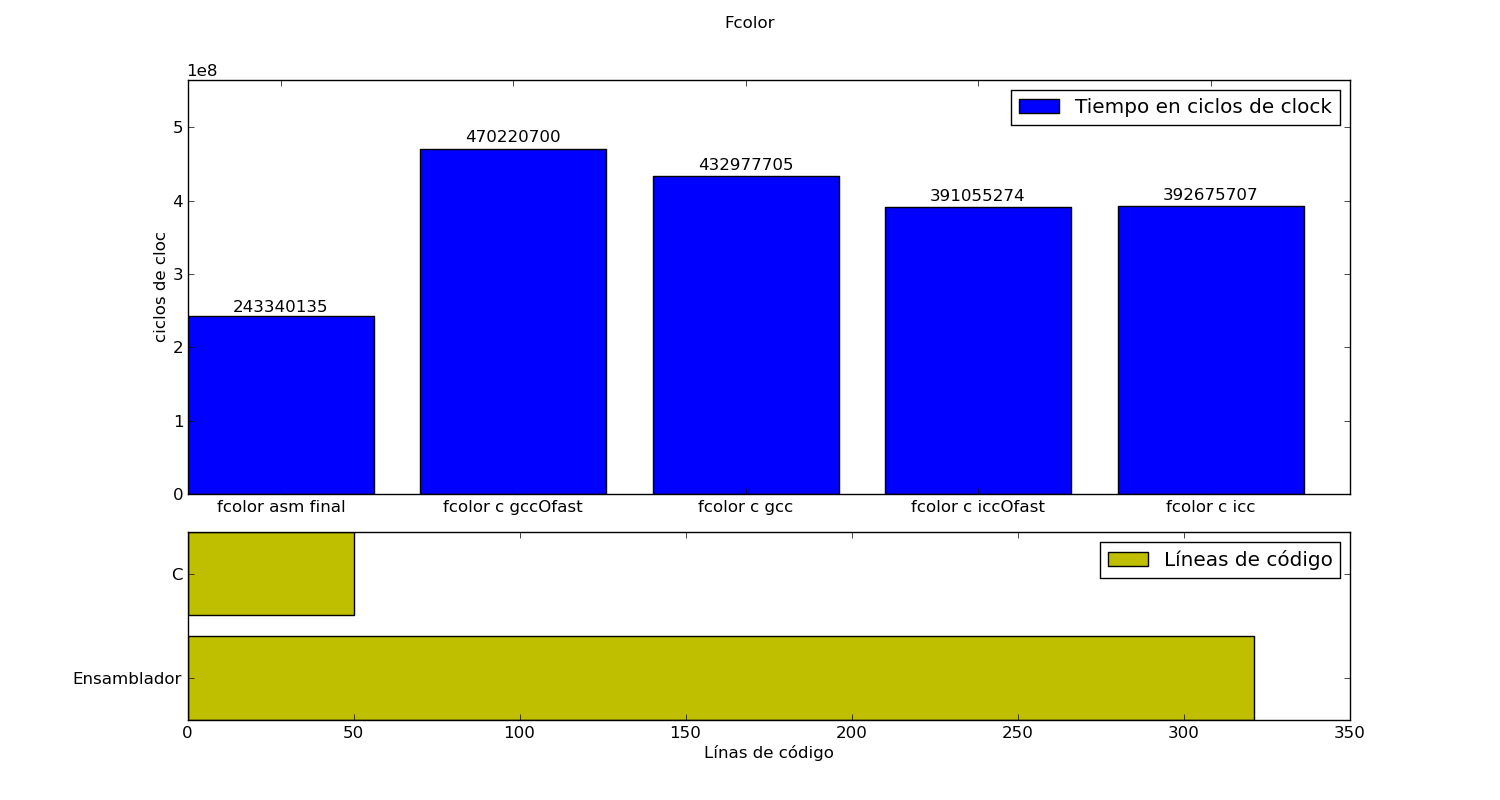
\includegraphics[scale=0.5]{secciones/filtro_color/graficos/fcolor.png}
\end{center}
\caption{Comparación de performance (superior) y cantidad de líneas de código (inferior) entre versión C básica y versión ASM básica.}
\label{fig:filtro-color-C-vs-ASM}
\end{figure}

El resultado muestra un incremento en velocidad de ejecución de aproximadamente 9 veces. Es importante destacar que esta mejora cercana a un orden de magintud no deviene de un cambio algorítmico, sino simplemente de un uso más provechoso de los recursos del procesador; particularmente, las operaciones SIMD. El costo de esta optimización recae en mayor tiempo de desarrollo, lo cual se puede retratar utilizando como indicador la cantidad de líneas de código mediante la figura \ref{fig:filtro-color-C-vs-ASM} (parte inferior).


\subsection{Optimizaciones en código C}
\label{sub:filtro-color-optimizaciones-c}

El código de la implementación en lenguaje C se compiló con distintos flags de optimización provistos por GCC. Estos son según la documentación de GCC \footnote{Ver http://gcc.gnu.org/onlinedocs/gcc/Optimize-Options.html.}:

\begin{itemize}
\item \textbf{-O/-O1}: Optimizar. Intentar reducir el tamaño de código y tiempo de ejecución sin realizar optimizaciones que requieran mucho tiempo de compilación.
\item \textbf{-O2}: Optimizar aún más. Se incrementa el tiempo de compilación y la performance del código generado. Esto incluye, por ejemplo, la eliminación del checkeo por punteros inválidos (delete-null-pointer-checks).
\item \textbf{-O3}: Optimizar incluso más. Incluye, por ejemplo, inlining automático de funciones y vectorización de loops (ftree-loop-vectorize).
\end{itemize}

Los resultados en cuestión de performance se pueden ver en la figura \ref{fig:filtro-color-C-vs-Os}, la cual muestra una comparación entre la cantidad de clocks consumidos durante la ejecución de cada versión.

\begin{figure}[H]
\begin{center}
  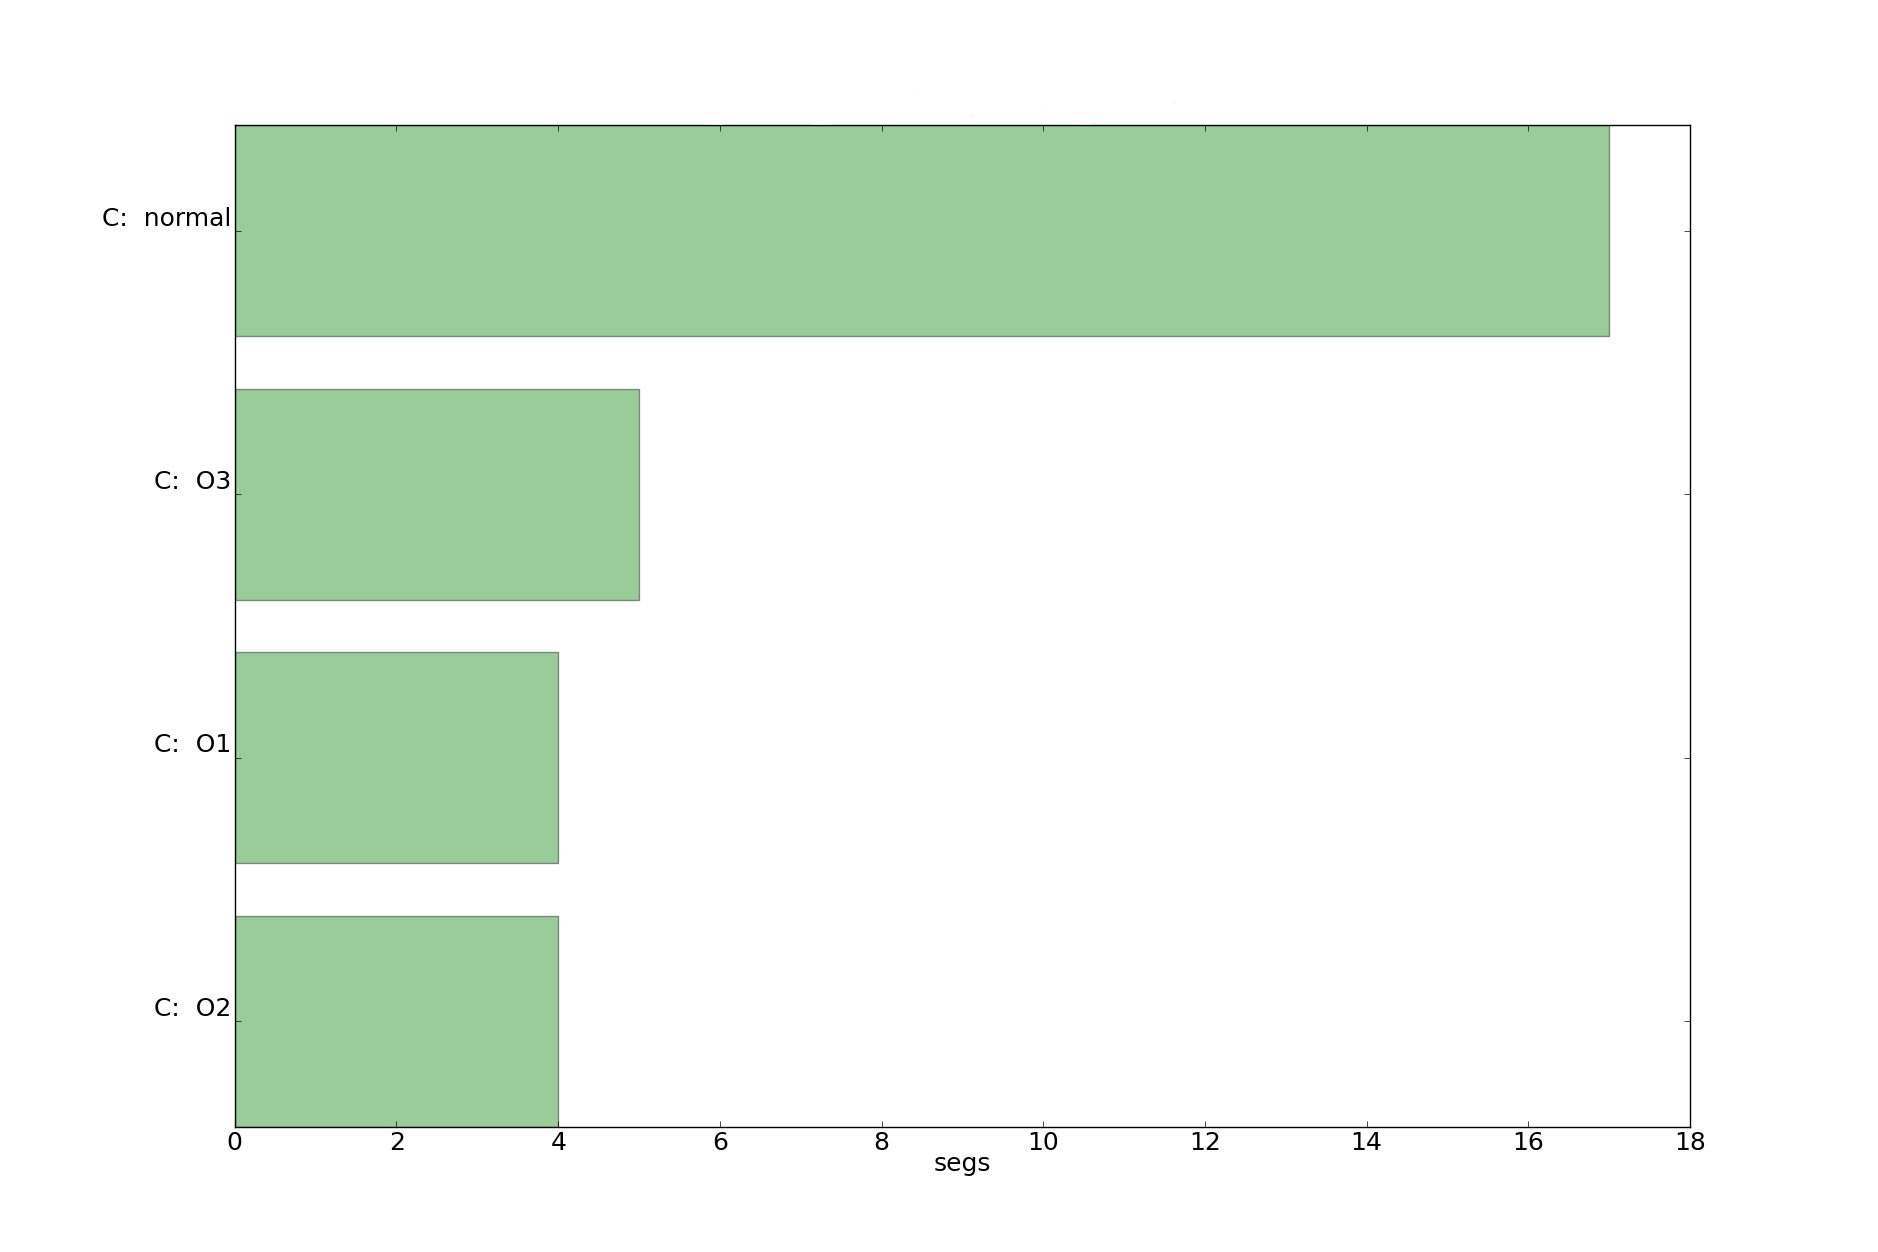
\includegraphics[scale=0.35]{secciones/filtro_color/graficos/C_normal_O1_O2_O3.png}
\end{center}
\caption{Comparación de performance entre la versión C compilada con distintos flags de optimización.}
\label{fig:filtro-color-C-vs-Os}
\end{figure}

El incremento en performance al activar las optimizaciones del compilador es notable, reduciendo a aproximadamente un cuarto el tiempo de ejecución en todos los casos. Sin embargo, la relación de performance entre los resultados con distintos flags no fue prevista; el flag \textbf{O3} generó código menos performante que las otras optimizaciones, y el flag \textbf{O2} fue muy levemente superior a la optimización de primer nivel. Esto permite aducir que los distintos tipos de optimización automática varían su utilidad según el código que se procesa, por lo cual siempre que se busque optimizar no es una buena estrategia optar por el mayor nivel de optimización \emph{sin realizar una comparación sobre el código particular que se desea optimizar.}

Adicionalmente, se analizaron las diferencias entre el código generado con compilación estándar y el código generado con optimización de tipo O1. La diferencia entre los códigos generados evidencia inmediatamente una característica subóptima del código estándar; \emph{todas} las variables locales se alojan en la pila, incluso habiendo disponibilidad de registros. Los registros se utilizan únicamente como variables temporales, y al final de cada extracto de código se guarda el resultado en un espacio de la pila. El código generado con O1, en cambio, ahorra gran cantidad de esos accesos a memoria. Este comportamiento se ejemplifica con el siguiente extracto (figura \ref{fig:codigo-objeto-filtro-color}).

% esto está atado con alambre...
\begin{figure}[h]
	\begin{mdframed}
	\begin{center}
		\begin{lstlisting}
		mov  eax, DWORD PTR[rbp-0x10]	| imul   r15d,r15d
		mov  edx,eax			| imul   r14d,r14d
		imul edx, DWORD PTR[rbp-0x10]	| add    r14d,r15d
		mov  eax, DWORD PTR[rbp-0xc]	| imul   ebx,ebx
		imul eax, DWORD PTR[rbp-0xc]	| add    ebx,r14d
		add  edx,eax			|			
		mov  eax, DWORD PTR[rbp-0x8]	|			
		imul eax, DWORD PTR[rbp-0x8]	|			
		add  eax,edx			|			
		mov  DWORD PTR [rbp-0x4],eax	|			
		\end{lstlisting}
	\end{center}
	\end{mdframed}
	\caption{Código objeto generado con compilación por default (izquierda), y con optimización de tipo O1 (derecha).}
	\label{fig:codigo-objeto-filtro-color}
\end{figure}

Sin embargo, la lógica de flujo del código generado es equivalente. Es decir, las operaciones realizadas y el orden en que se realizan son iguales; se mantiene la forma de recorrer la imagen y el procesamiento píxel por píxel.

%Análisis de saltos condicionales

\subsection{Análisis de saltos condicionales}

	Los saltos condicionales son algo absolutamente necesario en la programación.
Si bien existen técnicas para minimizarlos todo diclo $for$ o $while$ consta
básicamente de un salto condicional que se repite una gran cantidad de veces.

	Sin embargo los saltos condicionales que estamos analizando ahora no son
esos sino aquellos que se realizan en medio de la iteración para decidir
si la operación que se va a realizar va a ser una u otra. Es decir que lo
que estamos analizando es como impacta el uso de $if$ en la performance
del filtro.

	
	El primer experimento realizado, entonces, fue sencillamente comentar
el código perteneciente al if. Este análisis en realidad no es justo
ni significativo. Al hacer esto se está comparando un código
que realiza una operación contra otro que no la realiza.
No se obtiene la diferencia entre realizar y no realizar saltos
condicionales sino que se obtiene la diferencia entre realizar
o no realizar una operación completa. Por eso este experimento
se modificó de la siguiente forma:

	A esta altura es importante mencionar que el procesador tiene una enorme
cantidad de optimizaciones para que los saltos condicionales
tengan la máxima performance posible, por eso para realizar este
análisis fue importante tener en cuenta esas optimizaciones y buscar
casos donde le resulte dificil saber que rama del if tiene que tomar.

	Pensando en esto se armaron 2 videos patrón. Ambos consisten
en una imagen repetida en todos los frames del video, lo que
cambia es la imagen.
	En el \textit{patr0n negativo} lo que se hizo fue crear una imagen
que aturdiera lo máximo posible al sistema de predicción de saltos.
La imagen es basicamente una matriz de pixeles que tiene
intercalados blancos con negros de la isguiente manera.

\begin{center}
$
 \begin{pmatrix}
   000000 & FFFFFF & 000000 & FFFFFF & \cdots & 000000 & FFFFFF \\
   FFFFFF & 000000 & FFFFFF & 000000 & \cdots & FFFFFF & 000000 \\
   000000 & FFFFFF & 000000 & FFFFFF & \cdots & 000000 & FFFFFF \\
   FFFFFF & 000000 & FFFFFF & 000000 & \cdots & FFFFFF & 000000 \\
   000000 & FFFFFF & 000000 & FFFFFF & \cdots & 000000 & FFFFFF \\
   \vdots & \vdots & \vdots  & \vdots  & \ddots & \vdots  \\
   FFFFFF & 000000 & FFFFFF & 000000 & \cdots & FFFFFF & 000000 \\
   000000 & FFFFFF & 000000 & FFFFFF & \cdots & 000000 & FFFFFF \\
\end{pmatrix}
$
\end{center}

	La idea con este patrón es que obligatoriamente en una iteración
entra al una rama del if y en la siguiente entra a la otra (si se pasan
los parámetros adecuados).

	El siguiente patrón \textit{patrón positivo} consiste sencillamente en una
imagen blanca repetida durante todo el video. Ambos videos tienen
la misma duración.

	El experimento consiste en comparar cuanto tarda el filtro
en realizarse de manera absoluta (sobre TODA la imagen) sin un
condicional y con un condicional. La idea es comparar peso que 
tiene sólo el salto condicional, pero sólo el salto condicional. Para esto
lo que se hizo fue modificar el código C del filtro añadiendo un 
$else$ al $if$ exactamente igual al $then$. Es decir que la comparación
se realiza pero el resultado es el mismo. La operación siempre se hace.

	Luego se sacó el $if$ pero se dejó la operación. Es decir que acá
también se reliza si o si la operación, sin ninguna clase de condicional
dando vueltas.


\begin{figure}[h]
	\begin{mdframed}
	\begin{center}
		\begin{lstlisting}
		if (Cond) then:    | 
			OPERACION  | 
		else:              | OPERACION
			OPERACION  |
		endif              |
		\end{lstlisting}
	\end{center}
	\end{mdframed}
	\caption{Experimento 1}
	\label{fig:Experimento Saltos}
\end{figure}

	El siguiente gráfico muestra los resultados obtenidos en una ronda de test.
Algunas datos usados para sacar conclusiones no quedan plasmados en este gráfico sin
embargo se explican luego.

\begin{figure}[H]
\begin{center}
  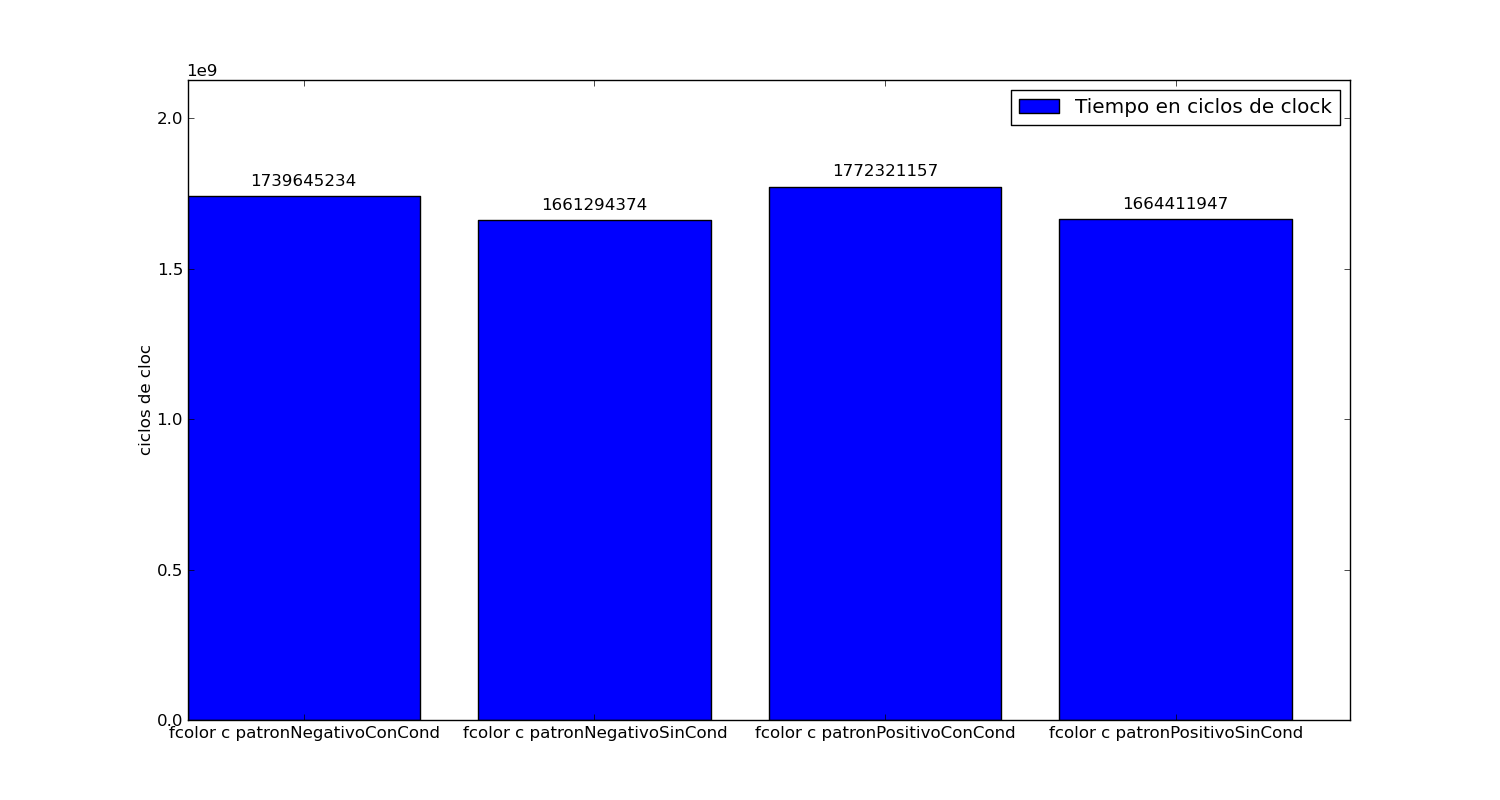
\includegraphics[scale=0.5]{secciones/filtro_color/graficos/performanceExpSaltos.png}
\end{center}
\caption{Resultados de una ronda de test del experimento de saltos}
\label{fig: Tiempos Experimento Saltos}
\end{figure}

	Si bien todas las baterías de test dieron resultados similares el análisis de todos
los resultados logró afirmar aún mas las conclusiones. A continuación
se detallan los comportamientos observados en los test y las concluiones obtenidas:

\begin{itemize}

	\item Como era de esperarse a la implementación sin condicionales no
le afecta la entrada. Es decir, el resultado obtenido para el patrón
positivo y para el patrón negativo fue el mismo. En algunas rondas de
test se realizó mas rápido uno y en otras otro. La diferencia de tiempo
es por cuestiones accidentales a la implementación en si.
	\item Como también era de esperar versión con $if$ resulta levemente
mas lenta. Los reultados oscilaron entre un 4\% y un 6\%. En principio
esto suena extraño, pues sencillamente se están ejecutando 2 o 3 instrucciones
extra para realizar el salto (recordemos que el condicional tiene el mismo código
en las 2 ramas del $if$). Es decir, se podría esperar que la diferencia sea menor.
Sin embargo lo qeu juega acá es el pipeline. Cuando hay condicionales
existen posibilidades de que el pipeline se rompa, además se invierte tiempo
en realizar las predicciones para no romper el pipeline. Esto explica esta diferencia.
	\item Lo mas interesante, tal vez, es la diferencia de tiempo entre
los dos patrones en la implementación con condicionales. Acá ambas ramas
del if son iguales, sin enbargo nos encontramos con una diferencia de performance que oscila
entre un 3\% y un 5\%. Esta diferencia si se vió de manera clara, en todas
las rondas de test el resultado fue el mismo. Eso muestra de manera bastante
que los saltos condicionales adquieren peso en la performance. Otra vez
la explicación de esto es el el pipeline. El patrón positivo es ``Pipeline Amigable'',
mientras que el patrón negitivo no lo es. Es decir el patrón negativo está pensado
para que se desarme el pipeline la mayor cantidad de veces posible.


\end{itemize}


\newpage

\subsection{Optimización en código ASM - Desenrollado de ciclos}
\label{sub:filtro-color-optimizaciones-asm}

Sobre la implementación en lenguaje ensamblador ya descripta, se realizaron dos sucesivas modificaciones para estudiar la técnica conocida como desenrollado de ciclos en su versión más elemental. Esta técnica consiste en minimizar la lógica de flujo, comparaciones y saltos condicionales para ciclos que realizan una gran cantidad de iteraciones. Un ejemplo esquemático se puede ver en la figura \ref{fig:filtro-color-loop-unrolling}.

\begin{figure}[h]
	\begin{mdframed}
	\begin{center}
		\begin{lstlisting}
		for i = 1 .. n		| for i = 1 .. n/k
			F(i)		| 	F(i)
		endfor			| 	F(i + 1)
					| 	...
					| 	F(i + k - 1)
					| endfor
		\end{lstlisting}
	\end{center}
	\end{mdframed}
	\caption{Pseudo-código ejemplo de la técnica loop unrolling.}
	\label{fig:filtro-color-loop-unrolling}
\end{figure}

Siguiendo la notación de la figura, en el caso particular del filtro color, se tomó k = 2, y k = 4, y se realizaron mediciones de performance. Los resultados no fueron provechosos ya que las mejoras observadas fueron menores al 5\%, incluso sin haber considerado el costo adicional de tratar con los casos donde el tamaño de la matriz no es múltiplo de la cantidad de píxeles que se procesan por ciclo, lo cual deterioraría la performance. Este resultado parecería indicar que el costo de la comparación y la escritura al program counter en cada salto no incurren un costo significativo, posiblemente debido a que el procedimiento realiza un único acceso a memoria por iteración (no congestiona la caché) y la posibilidad de ejecución fuera de orden que brinda al procesador (el puntero de lectura que se utiliza para realizar la comparación no se utiliza dentro del cuerpo del ciclo una vez leída la memoria).
